\chapter{Framework}
\label{sec:framework}
The current state-of-the-art tools for cyber-physical systems focus on individual aspects of testing, such as network or hardware simulation, but are siloed from other tools. Many other tools and platforms exist that could support these CPS tools with other aspects of CPS testing, such as environment and physics simulation, formal modelling, or statistical analysis tools, without the need to directly extend or integrate these features within any of them. 

Hence, the goal of this framework is to provide an open, stable and extensible platform into which a variety of tools can be integrated to support the simulation, testing, modelling and analysis of cyber-physical systems.

This section proposes an architecture for designing a distributed framework supporting a co-simulation approach for testing and analysis of cyber-physical systems using multiple tools.
This will enhance the information sharing between tools, enabling developers to seamlessly use these tools in tandem and close the loop, e.g., 3D simulator updates positions of devices based on physical interaction with the virtual world, this is then reflected in the network simulator which affects the radio transmission range and interference.

\section{Architecture and Communication} % (fold)
\label{sub:architecture}
Rather than integrate different co-simulation components together directly, our approach uses a publish/subscribe event bus and common schema to describe information passed between the different tools. This approach reduces the tight coupling between tools, allowing for individual tools to be removed, added or replaced with minimal configuration. We envision the integration of tools such as model checking, statistical analysis, unit-testing and advanced simulation for radio and environmental properties.

Each tool publishes or subscribes to the relevant topics of interest within the event stream, enabling other tools to observe or inform one another of events in a many-to-many fashion. Typically, only one tool will publish data to a topic related to that which it specialises in, e.g., radio simulator publishes when transmissions were sent and received. Other tools subscribed to this stream may then publish a composite event, adding more data, analysis or context back to the event stream.

To support the platform each tool needs to build a plugin which communicates between the event bus and tool itself, subscribing to and publishing data. A tool's plugin defines a set of topics to which it publish/subscribe to, providing developers with a clear interface between co-operating tools.
% subsection architecture (end)
\begin{figure}[ht]
\centering
  % \includesvg[svgpath = ./imgs/, width = 0.5\textwidth]{architecture}
  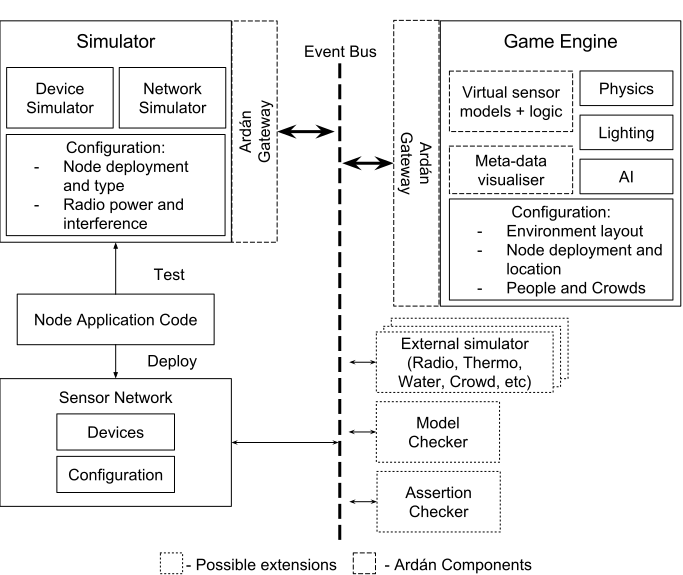
\includegraphics[width=\textwidth]{./imgs/architecture}
  \caption{Ard\'{a}n architecture}
  \label{fig:architecture}
\end{figure}



\section{Time} % (fold)
\label{sub:time}
Within the simulation world there are two clocks, the simulated time and the real world or wall clock time, how much time has passed in the simulation reality and how much time has passed the the real world. Comparing these two times gives us the simulation rate, i.e., how much simulated time passes in 1 second of real world time. It's often the case that simulations can run faster than real-time, resulting in a simulation rate >1x, providing results faster than had they been carried out in the real world. Similarly, users can also select to run simulations slower than real-time, giving developers more time to observe and analyse the simulation in real-time.

When performing co-simulation between different components or tools, it's necessary to ensure the simulation tools remain synchronised, such that the individual simulations aren't adversely affected, e.g., the CPS simulation lags behind the virtual world simulation, resulting in delayed and slow CPS response times, causing devices in the virtual world to actuate incorrectly.

Also, should a developer choose to run a simulation at a speed faster or slower than real-time, it is also necessary to ensure the co-simulation tools support this functionality and are instructed to simulate at the desired speed.
% subsection time (end)

\subsection{Human Mobility} % (fold)
\label{sub:human_mobility}
Within Ardan, the game engine component is responsible for human mobility, handling the physical modelling and characteristics, such as size, weight, speed and appearance, as well as their behaviours.

When creating a virtual person, henceforth referred to as a agent, developers can choose to create or spawn them in one of three ways: programmatically in C++, spawning an agent specifying their appearance, scale (size) and location; interactively, using the visual game engine editor to select a agent type, drag and then drop into the environment, before then assigning further attributes; scripting in the game engine's visual programming tool, similar to C++ in its API and programming logic, however, it provides developers with a visual drag-and-drop based programming tool, with useful auto-suggestions and completion.

Utilising the physics engine within the game, an agent's properties, such as size and weight, can have a significant impact on their interactivity with the world, such as their body fitting through spaces or their weight impacting their momentum and force in collisions with other objects. To navigate the physical environment, agents use a navigation mesh built by the physics engine, which calculates traversable paths for agents to use to navigate within the environment, around obstacles, through doorways and up ramps or stairs. Agents then use the A* algorithm on the navigation mesh to find the shortest path to their destination.

After spawning an agent, behaviours can be assigned to them which they will perform at run-time. Behaviours, similar to spawning an agent, can be created and customised using the previously mentioned methods. The visual programming tool simplifies this process, by enabling developers to interactively find and select entities of interest and create sequences of conditions and actions to form behaviours. Developers have access to a large API of primitives to support complex behaviours, such as sphere and ray tracing, used to detect and measure nearby and visible agents or entities. Behaviours can be as simple as move to a location, requiring an agent to navigate the environment and avoid any obstacles; or more complex, such as agent X follow agent Y, requiring the agent X to determine where Y is before than navigating to their position. 

Agents 

It is also possible to create crowd behaviours, such as herding, in which a group of agents move and perform actions as a collective unit, without any central decision making. These behaviours can be constructed by creating agent behaviours that are influenced by other agents and their behaviours. Within the game engine a  herd may start due to an agent following someone who they deem has authority in a situation (manager, teacher). The herd may also influence other agents to join in due size of the group, 'flocking'. For example, within a fire evacuation a manager may form a herd with colleagues leading them to a safe exit, other agents observing would choose to follow even if the route was neither the safest nor quickest.

Group behaviour, family/friends waiting/searching

Occupant aggression, physiological differences

% subsection human_mobility (end)